\begin{frame}[fragile]{Monad}
	\begin{textblock*}{5cm}(1cm,1.45cm)
		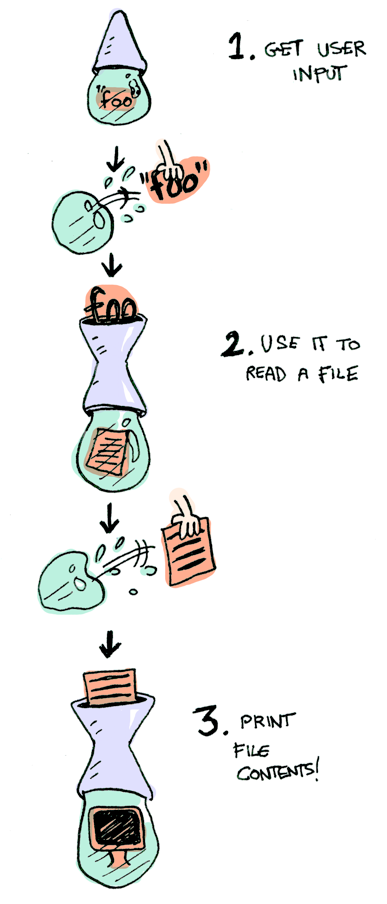
\includegraphics[scale=0.23]{monad}
	\end{textblock*}
	\begin{textblock*}{5cm}(5cm,3cm)
		\begin{itemize}
			\item It chains operations in some specific, useful way
			\item Everything is based on a \textbf{bind} operator
			\begin{itemize}
				\item Applies a function that returns a wrapped value to a wrapped value
			\end{itemize}
		\end{itemize}
		\begin{onlyenv}<2->
			\begin{lstlisting}
				getLine >>= readFile >>= putStrLn
			\end{lstlisting}
		\end{onlyenv}
	\end{textblock*}
\end{frame}